%%%%%%%%%%%%%%%%%%%%%%%%%%%%%%%%%%%%%%%%%
% Frequently Asked Questions
% LaTeX Template
% Version 1.0 (22/7/13)
%
% This template has been downloaded from:
% http://www.LaTeXTemplates.com
%
% Original author:
% Adam Glesser (adamglesser@gmail.com)
%
% License:
% CC BY-NC-SA 3.0 (http://creativecommons.org/licenses/by-nc-sa/3.0/)
%
%%%%%%%%%%%%%%%%%%%%%%%%%%%%%%%%%%%%%%%%%

\documentclass[11pt]{article}

\usepackage[margin=1in]{geometry} % Required to make the margins smaller to fit more content on each page
\usepackage[linkcolor=blue]{hyperref} % Required to create hyperlinks to questions from elsewhere in the document
\hypersetup{pdfborder={0 0 0}, colorlinks=true, urlcolor=blue} % Specify a color for hyperlinks
\usepackage{todonotes} % Required for the boxes that questions appear in
\usepackage{tocloft} % Required to give customize the table of contents to display questions
\usepackage{microtype} % Slightly tweak font spacing for aesthetics
\usepackage{palatino} % Use the Palatino font



\usepackage[utf8]{inputenc} 
\usepackage[french]{babel} 



\usepackage{listings} % Required for inserting code snippets


\lstdefinestyle{customc}{
  belowcaptionskip=1\baselineskip,
  breaklines=true,
  frame=L,
  xleftmargin=\parindent,
  language=C,
  showstringspaces=false,
  basicstyle=\footnotesize\ttfamily,
  keywordstyle=\bfseries\color{green!40!black},
  commentstyle=\itshape\color{purple!40!black},
  identifierstyle=\color{blue},
  stringstyle=\color{orange},
}

\lstdefinestyle{customasm}{
  belowcaptionskip=1\baselineskip,
  frame=L,
  xleftmargin=\parindent,
  language=[x86masm]Assembler,
  basicstyle=\footnotesize\ttfamily,
  commentstyle=\itshape\color{purple!40!black},
}

\lstset{escapechar=@,style=customc}


\setlength\parindent{0pt} % Removes all indentation from paragraphs

% Create and define the list of questions
\newlistof{questions}{faq}{\large List of Frequently Asked Questions} % This creates a new table of contents-like environment that will output a file with extension .faq
\setlength\cftbeforefaqtitleskip{4em} % Adjusts the vertical space between the title and subtitle
\setlength\cftafterfaqtitleskip{1em} % Adjusts the vertical space between the subtitle and the first question
\setlength\cftparskip{.3em} % Adjusts the vertical space between questions in the list of questions

% Create the command used for questions
\newcommand{\question}[1] % This is what you will use to create a new question
{
\refstepcounter{questions} % Increases the questions counter, this can be referenced anywhere with \thequestions
\par\noindent % Creates a new unindented paragraph
\phantomsection % Needed for hyperref compatibility with the \addcontensline command
\addcontentsline{faq}{questions}{#1} % Adds the question to the list of questions
\todo[inline, color=blue!40]{\textbf{#1}} % Uses the todonotes package to create a fancy box to put the question
\vspace{1em} % White space after the question before the start of the answer
}

% Uncomment the line below to get rid of the trailing dots in the table of contents
%\renewcommand{\cftdot}{}

% Uncomment the two lines below to get rid of the numbers in the table of contents
%\let\Contentsline\contentsline
%\renewcommand\contentsline[3]{\Contentsline{#1}{#2}{}}



\begin{document}

%----------------------------------------------------------------------------------------
%	TITLE AND LIST OF QUESTIONS
%----------------------------------------------------------------------------------------

\begin{center}
\Huge{\bf \emph{NoSQL 2015 \\ TD 1}} % Main title
\end{center}

\begin{center}
Professeurs 

\bigskip 


Houda Chabbi Drissi \\et \\Benoît Perroud \\
\end{center}

\begin{center}
\begin{figure}[h!]

  \centering
    
\includegraphics[width=0.4\textwidth]{Images/Logo_HEIA-FR_site}
     
\end{figure}
\end{center}



\begin{figure}[h!]

  \centering
    
\includegraphics[width=1\textwidth]{Images/Hadoop-tutorial.png}
     
\end{figure}

\bigskip

\begin{center}
 


\begin{figure}[h!]

  \centering
    
\includegraphics[width=0.5\textwidth]{Images/DAPLab-Title.png}
     
\end{figure}
\end{center}


\begin{center} 
Assistant : Christophe Bovigny
\end{center}

\listofquestions % This prints the subtitle and a list of all of your questions

\newpage % Comment this if you would like your questions and answers to start immediately after table of questions

%----------------------------------------------------------------------------------------
%	QUESTIONS AND ANSWERS
%----------------------------------------------------------------------------------------

% \question{Prérequis}\label{new-question}
% 
% 
% Tous les étudiants doivent envoyer une clé publique ssh à l'addresse email : bovignyc@gmail.com afin de pouvoir se connecter et s'exercer sur le cluster DAPLAB
% \\
% Génération de la clé publique:
% \\
% \lstinputlisting[language=sh]{Scripts/sshkey.sh}
% 
% Clé à envoyer :
% \\
% \lstinputlisting[language=sh]{Scripts/seekey.sh}
% 
% Connection au Cluster :
% 
% Votre login est la première lettre de votre prenom suivi par votre nom : (Exemple : Christophe Bovigny = cbovigny). Durant ce travail dirigé tous les exemples seront produits 
% avec l'utilisateur cbovigny. 
% %\lstinputlisting[language=Python]{Scripts/login.sh}
% 
% \lstinputlisting[language=sh,mathescape]{Scripts/login.sh}
%  % The first argument is the script location/filename and the second is a caption for the listing
% %\begin{verbatim}
% %\question{A question that needs answering}\label{question-label}
% 
% %The answer to this question.
% %\end{verbatim}

%------------------------------------------------

%\question{Why is there a label in the code for \hyperref[new-question]{the previous question}?}\label{labels}


\question{HDFS (Hadoop Distributed File System)}\label{new-question}

\begin{center}
{\bf \emph{Manipuler des répertoires dans HDFS}} % Main title
\end{center}

Tout d'abord nous allons créer un répertoire TD1 dans le système de fichier HDFS.
\lstinputlisting[language=sh,mathescape]{Scripts/createdirectoryhdfs.sh}
Créez un sous-répertoire EX1 dans TD1.
%%%%%%%%%%%%%%%%%%%%%%%%% SOLUTION 1%%%%%%%%%%%%%%%%%%%%%%%%%%%%%%%%
\lstinputlisting[language=sh,mathescape]{Scripts/createex1hdfs.sh}
%%%%%%%%%%%%%%%%%%%%%%%%%%%%%%%%%%%%%%%%%%%%%%%%%%%%%%%%%%%%%%%%%%%%

Listez tous les fichiers et répertoire de votre home.
\lstinputlisting[language=sh,mathescape]{Scripts/listhdfs.sh}

Vous devriez y voir votre dossier TD1 fraîchement créé.

\lstinputlisting[language=sh,mathescape]{Scripts/viewhdfsls.sh}

Maintenant listez récursivement vos dossier afin de voir le dossier EX1 qui se trouve dans TD1.(Astuce : Utilisez l'option -R)

\lstinputlisting[language=sh,mathescape]{Scripts/viewhdfslsR.sh}

%%%%%%%%%%%%%%%%%%%%%%%%% SOLUTION 2%%%%%%%%%%%%%%%%%%%%%%%%%%%%%%%%
Solution :
\lstinputlisting[language=sh,mathescape]{Scripts/viewhdfslsRsolution.sh}
%%%%%%%%%%%%%%%%%%%%%%%%%%%%%%%%%%%%%%%%%%%%%%%%%%%%%%%%%%%%%%%%%%%%


Effacez les deux dossiers TD1 et EX1 créés précédement en une seule commande :

\lstinputlisting[language=sh,mathescape]{Scripts/eraseall.sh}

Et à nouveau créer un dossier et sous-dossier TD1/EX1 mais cette fois-ci en une seule commande

\lstinputlisting[language=sh,mathescape]{Scripts/mkdirp.sh}


{\bf \emph{Créer un dossier et un sous-dossier TD1\_LOCAL et EX1\_LOCAL, mais cette fois-ci en utilisant que les commandes linux standard et en n'employant pas le système de fichier HDFS }} % Main title

\paragraph{}
\begin{center}


{\bf \emph{Manipuler des fichiers dans HDFS}} % Main title
\end{center}
Allez dans le répertoire EX1\_LOCAL et téléchargez le fichier data.txt à l'addresse suivante :


\lstinputlisting[language=sh,mathescape]{Scripts/download.sh}

\lstinputlisting[language=sh,mathescape]{Scripts/viewdownload.sh}

Nous allons transférer le fichier data.txt de notre dossier local : \\
\textit{/votrehome/TD1\_LOCAL/EX1\_LOCAL/data.txt}

dans le répertoire EX1 du système de fichier HDFS 

\textit{TD1/EX1/} 

(Astuce : Pour ceci utilisez la commande copyFromLocal) \\
\bigskip
\bigskip
\bigskip

Solution :
%%%%%%%%%%%%%%%%%%%%%%%%% SOLUTION 3%%%%%%%%%%%%%%%%%%%%%%%%%%%%%%%%
\lstinputlisting[language=sh,mathescape]{Scripts/copyfromlocal.sh}
%%%%%%%%%%%%%%%%%%%%%%%%%%%%%%%%%%%%%%%%%%%%%%%%%%%%%%%%%%%%%%%%%%%%

Afin de voir le contenu du fichier data.txt se trouvant dans le système de fichier HDFS, vous pouvez utiliser la commande cat :

\lstinputlisting[language=sh,mathescape]{Scripts/cat.sh}

Nous allons effacer le fichier local data.txt et ensuite copier le fichier data.txt de HDFS en Local


\lstinputlisting[language=sh,mathescape]{Scripts/copytolocal.sh}

Exercice :
Downloader en Local deux fichiers via les commandes ci-dessous dans le repertoire /votrehome/TD1\_LOCAL/EX1\_LOCAL/FILES\_LOCAL/:

\lstinputlisting[language=sh,mathescape]{Scripts/download2.sh}

Créez un répertoire TD1/EX1/FILES sous HDFS et copiez les fichiers part-m-00000 et part-m-00001 à l'intérieur de ces derniers.
\bigskip
\bigskip
\bigskip

Solution :
%%%%%%%%%%%%%%%%%%%%%%%%% SOLUTION 4%%%%%%%%%%%%%%%%%%%%%%%%%%%%%%%%
\lstinputlisting[language=sh,mathescape]{Scripts/copyfromlocal2files.sh}
%%%%%%%%%%%%%%%%%%%%%%%%%%%%%%%%%%%%%%%%%%%%%%%%%%%%%%%%%%%%%%%%%%%%

Après cet exercice il serait intéressant de concaténer ces deux fichiers en un et de les analyser en local. hdfs dfs -getmerge permet de tout faire en une seule commande. 
Une petite variante existe, si vous désirez insérer une ligne vide dans le fichier final entre chaque fichiers concaténés, ajouter l'option -nl 

\lstinputlisting[language=sh,mathescape]{Scripts/getmerge.sh}


\begin{figure}[h!]

  \centering
    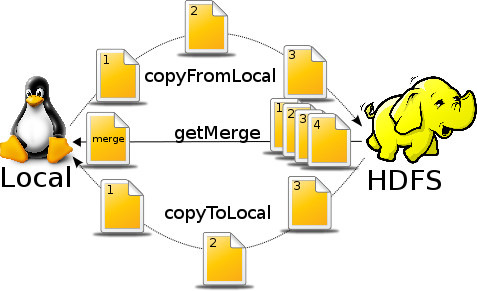
\includegraphics[width=0.5\textwidth]{Images/drawing.jpg}
      \caption{copyFromLocal/copyToLocal/getmerge}
\end{figure}


\begin{center}
{\bf \emph{Grandeur de Block dans HDFS}} % Main title
\end{center}

Effacez le fichier part-m-00000 dans hdfs avec la commande appropriée et ensuite essayez de le remettre avec un blocksize de 30 bytes. (Astuce : placez l'option -D dfs.blocksize=bytesize juste après hdfs dfs)

Réponse:(Message affiché en sortie de la commande et expliquez) :

\bigskip
\bigskip
\bigskip


Solution:
%%%%%%%%%%%%%%%%%%%%%%%%%%%%%%%%%%%%%%%%%%%%%%%%%%%%%%%%%%%%%%%%%%%%
\lstinputlisting[language=sh,mathescape]{Scripts/blocksize30.sh}
%%%%%%%%%%%%%%%%%%%%%%%%%%%%%%%%%%%%%%%%%%%%%%%%%%%%%%%%%%%%%%%%%%%%


\question{Map/Reduce}\label{new-question}

Dans cette partie, nous allons essayer de comprendre comment fonctionne le map/reduce de Hadoop. Ce dernier a pour but de compter la fréquence de chaque mots dans un ou plusieurs
fichiers textes.

Le programme a plusieurs sections, la première partie est composée de la classe MapClass. Que fait-elle et que retourne-t-elle ?



\lstinputlisting[language=java]{Scripts/Map.java}



La deuxième partie est naturellement la classe Reduce. Comme précédement veuillez commenter et expliquer que fait cette classe ?


\lstinputlisting[language=java]{Scripts/Reduce.java}


Voici le code source final:

\lstinputlisting[language=java]{Scripts/WordCount.java}



Maintenant nous allons exécuter ce programme sous le cluster Hadoop du DAPLAB. Connectez-vous au cluster et ensuite créer un répertoire TD1\_MAPREDUCE dans votre home.
Ensuite copiez les deux fichiers 4300.txt et hadoop-0.20.1-examples.jar dans ce répertoire précédement créer. 
\paragraph{}

Le pas d'après sera de placer le fichier 4300.txt dans un répertoire HDFS qui se nommera également TD1\_MAPREDUCE. (CF:exercice 1)
\paragraph{}
Ensuite lancez la commande :


\lstinputlisting[language=sh,mathescape]{Scripts/launchmapreduce.sh}


Veuillez transférer le resultat obtenu de HDFS en local et commentez l'output obtenu.






% \question{Prérequis}\label{new-question}
% This is not necessary, but it does give you a way of linking to a different question. In order to link to another question you simply need to add the following:
% 
% 
% 
% 
% 
% \begin{verbatim}
% \hyperref[question-label]{click here}
% \end{verbatim}
% 
% The first part \texttt{[question-label]} is the label name and the second part \texttt{\{click here\}} is the text that is displayed as link.
% 
% %------------------------------------------------
% 
% \question{How do I change the title and subtitle?}\label{change-title}
% 
% To change the main title, simply find the "TITLE AND LIST OF QUESTIONS" block and replace "A Template for FAQ's" within it. To change the subtitle find the following command:
% 
% \begin{verbatim}
% \newlistof{questions}{faq}{\large List of Frequently Asked Questions}
% \end{verbatim}
% 
% and replace the subtitle with one of your choosing.
% 
% %------------------------------------------------
% 
% \question{Is it possible to change the spacing between the questions in the list of questions?}\label{change-spacing}
% 
% Yes, simply find the following line:
% 
% \begin{verbatim}
% \setlength\cftparskip{.3em}
% \end{verbatim}
% 
% and change the \texttt{.3em} to whatever suits your fancy.
% 
% %------------------------------------------------
% 
% \question{What if I want to hide the page numbers and/or trailing dots next to the question in the list of questions?}\label{page-numbering}
% 
% To remove the trailing dots to the page numbers, find the line:
% 
% \begin{verbatim}
% %\renewcommand{\cftdot}{}
% \end{verbatim}
% and uncomment it. To remove the page numbers as well, find the following lines and uncomment them:
% \begin{verbatim}
% %\let\Contentsline\contentsline
% %\renewcommand\contentsline[3]{\Contentsline{#1}{#2}{}}
% \end{verbatim}
% 
% %------------------------------------------------
% 
% \question{Is it possible to number questions?}\label{number-questions}
% 
% Yes, you can refer to the number of the current question with:
% 
% \begin{verbatim}
% \thequestions
% \end{verbatim}
%  
% For example, this is question \thequestions. You can even incorporate question numbers into the questions and list of questions automatically by adding:
% 
% \begin{verbatim}
% Question \thequestions:
% \end{verbatim}
% 
% just before each \texttt{\#1} in the \texttt{\textbackslash questions} definition block in the preamble.
% 
% %------------------------------------------------
% 
% \question{Question \thequestions: Can I change the color of the question boxes?}\label{question-color}
% 
% Just find the following line and change the color specified there:
% 
% \begin{verbatim}
% \todo[inline, color=green!40]{\textbf{#1}}
% \end{verbatim}
% 
% %----------------------------------------------------------------------------------------

\end{document}